\documentclass[12pt]{article}
\usepackage[utf8]{inputenc}
\usepackage{amsmath,amssymb,amsthm}
\usepackage{graphicx}
\usepackage{listings}
\usepackage{xcolor}
\usepackage{hyperref}
\usepackage{geometry}
\geometry{margin=1in}
\usepackage{float}

\title{Domácí úkol 07}
\author{Jáchym Kouba}
\date{\today}

% Add a dot after section numbers
\renewcommand{\thesection}{\arabic{section}.}

% MATLAB listings setup
\lstdefinestyle{mystyle}{
  language=Matlab,
  basicstyle=\ttfamily\small,
  keywordstyle=\color{blue},
  commentstyle=\color{gray},
  stringstyle=\color{teal},
  numbers=left,
  numberstyle=\tiny\color{gray},
  stepnumber=1,
  numbersep=8pt,
  tabsize=2,
  breaklines=true,
  showstringspaces=false
}
\lstset{style=mystyle}

\begin{document}
\maketitle

\newpage

\section{Příklad 1}

\begin{figure}[H]
    
\includegraphics[width=1\textwidth]{notebook1.jpg}
    \caption{zápisky 1}
\end{figure}

\begin{figure}[H]
    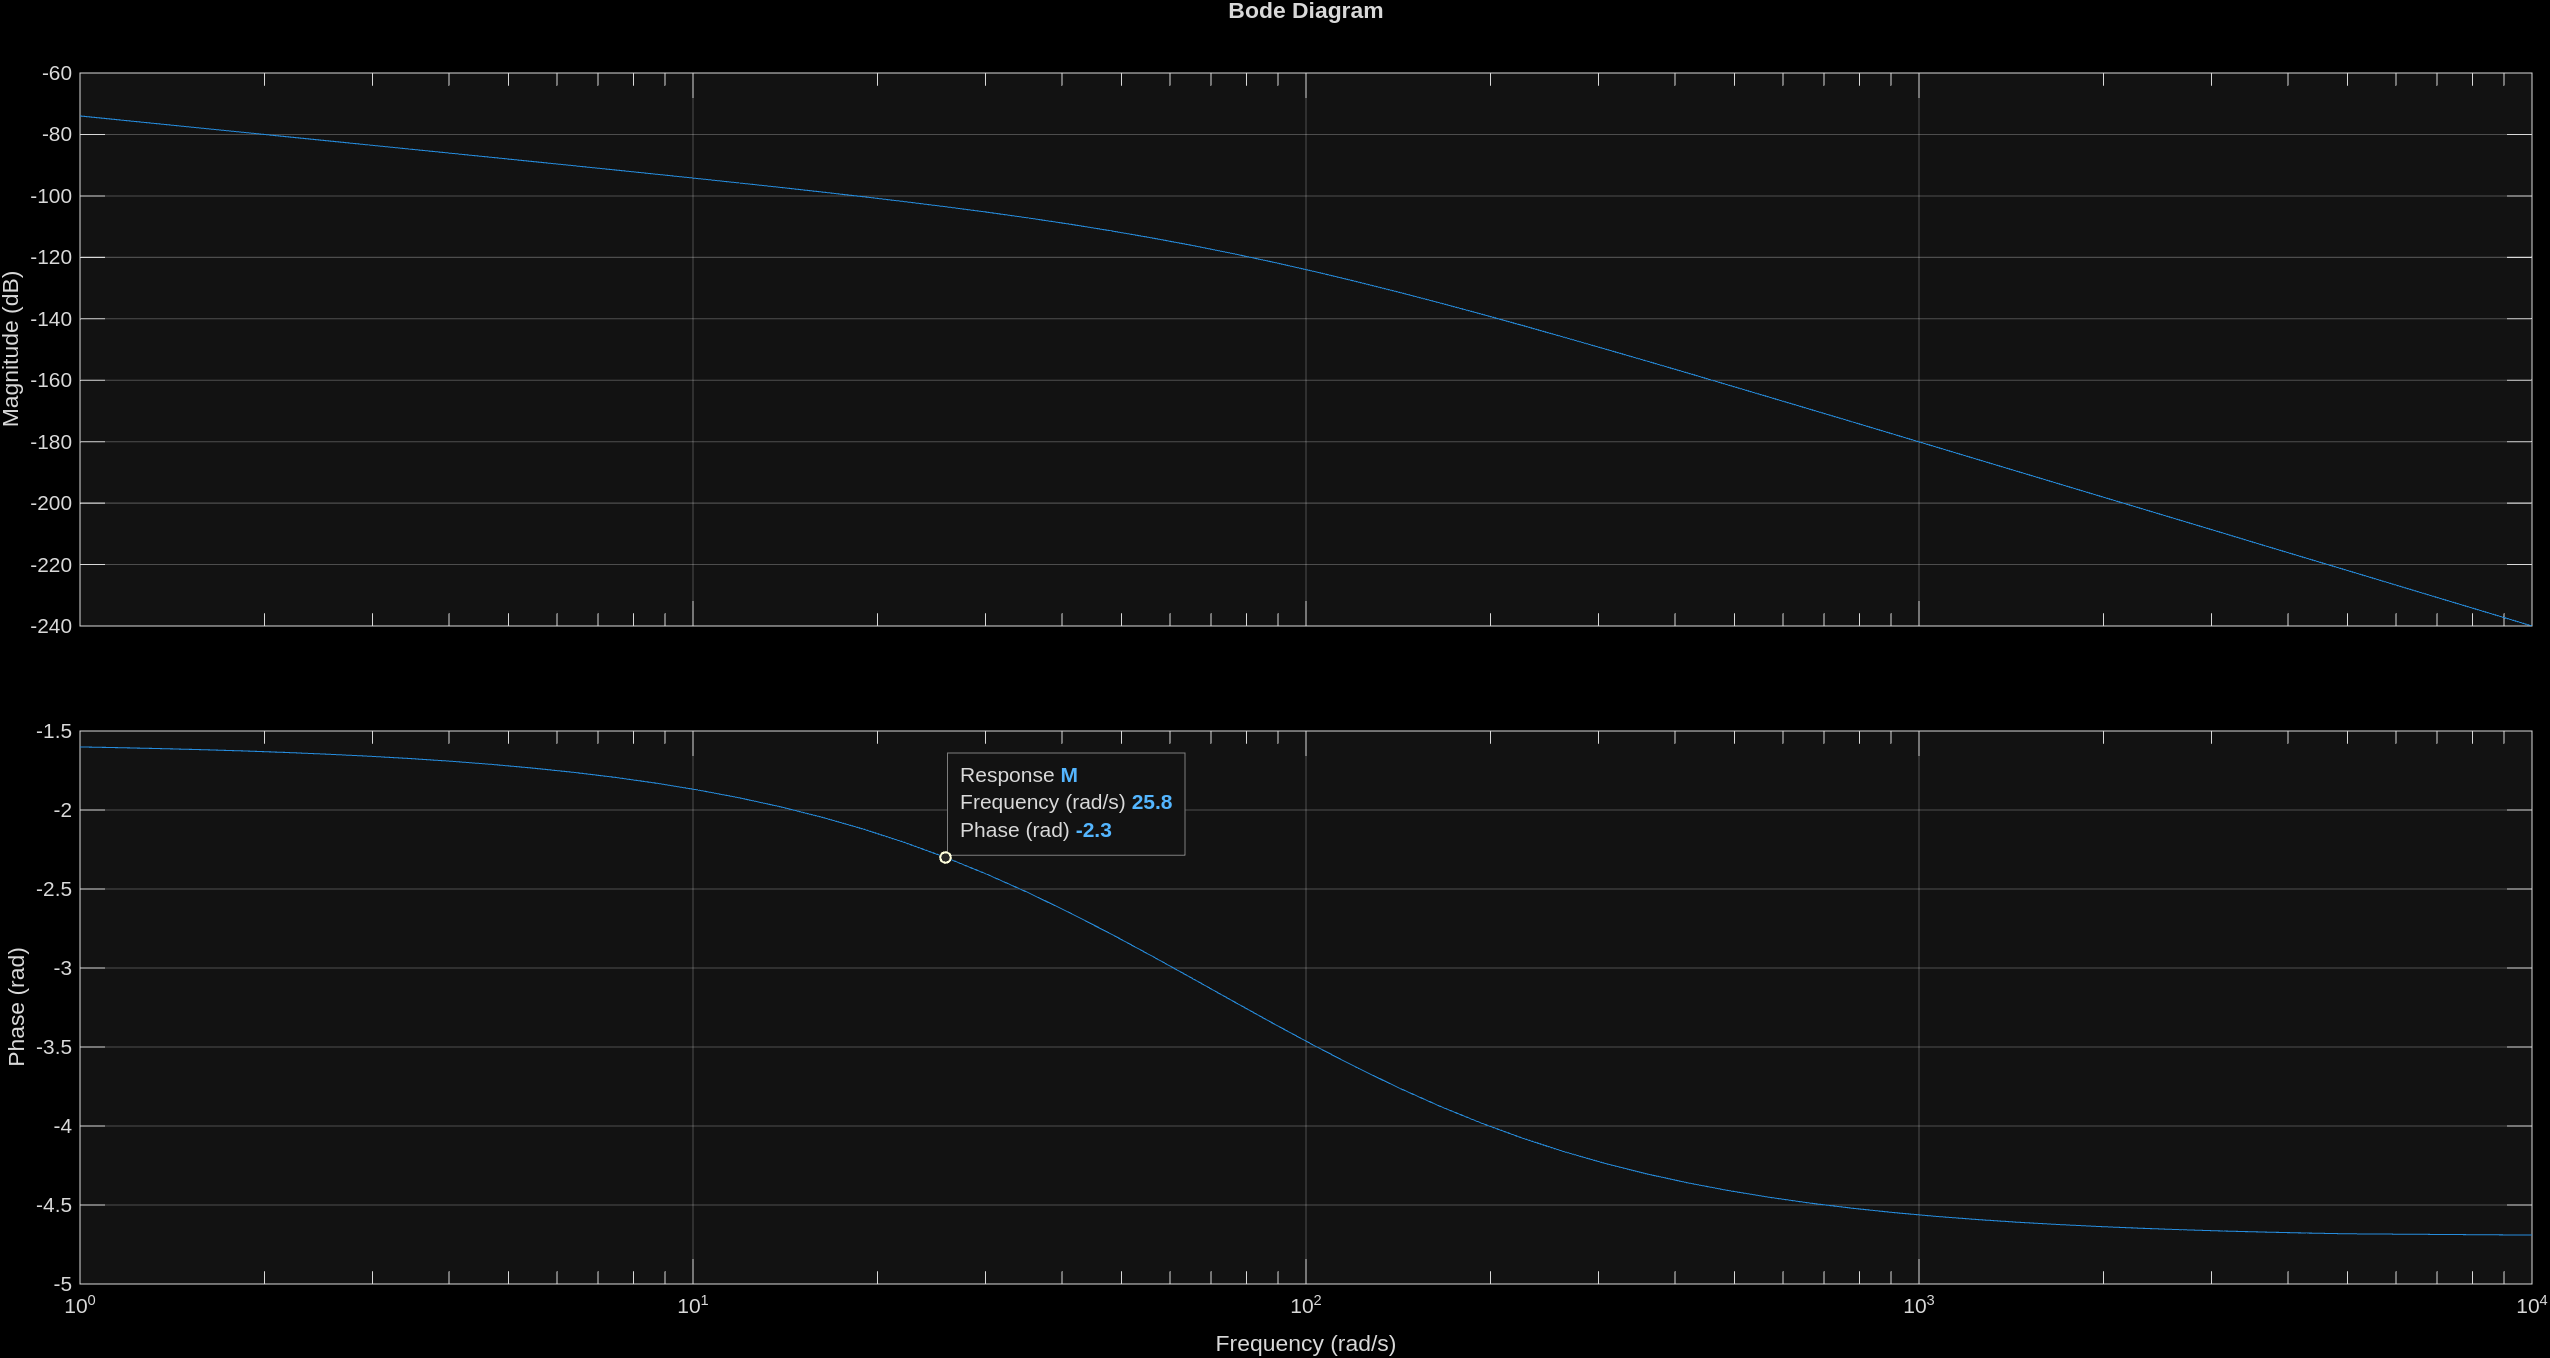
\includegraphics[width=1\textwidth]{bode.png}
    \caption{bode}
\end{figure}
\begin{figure}[H]
    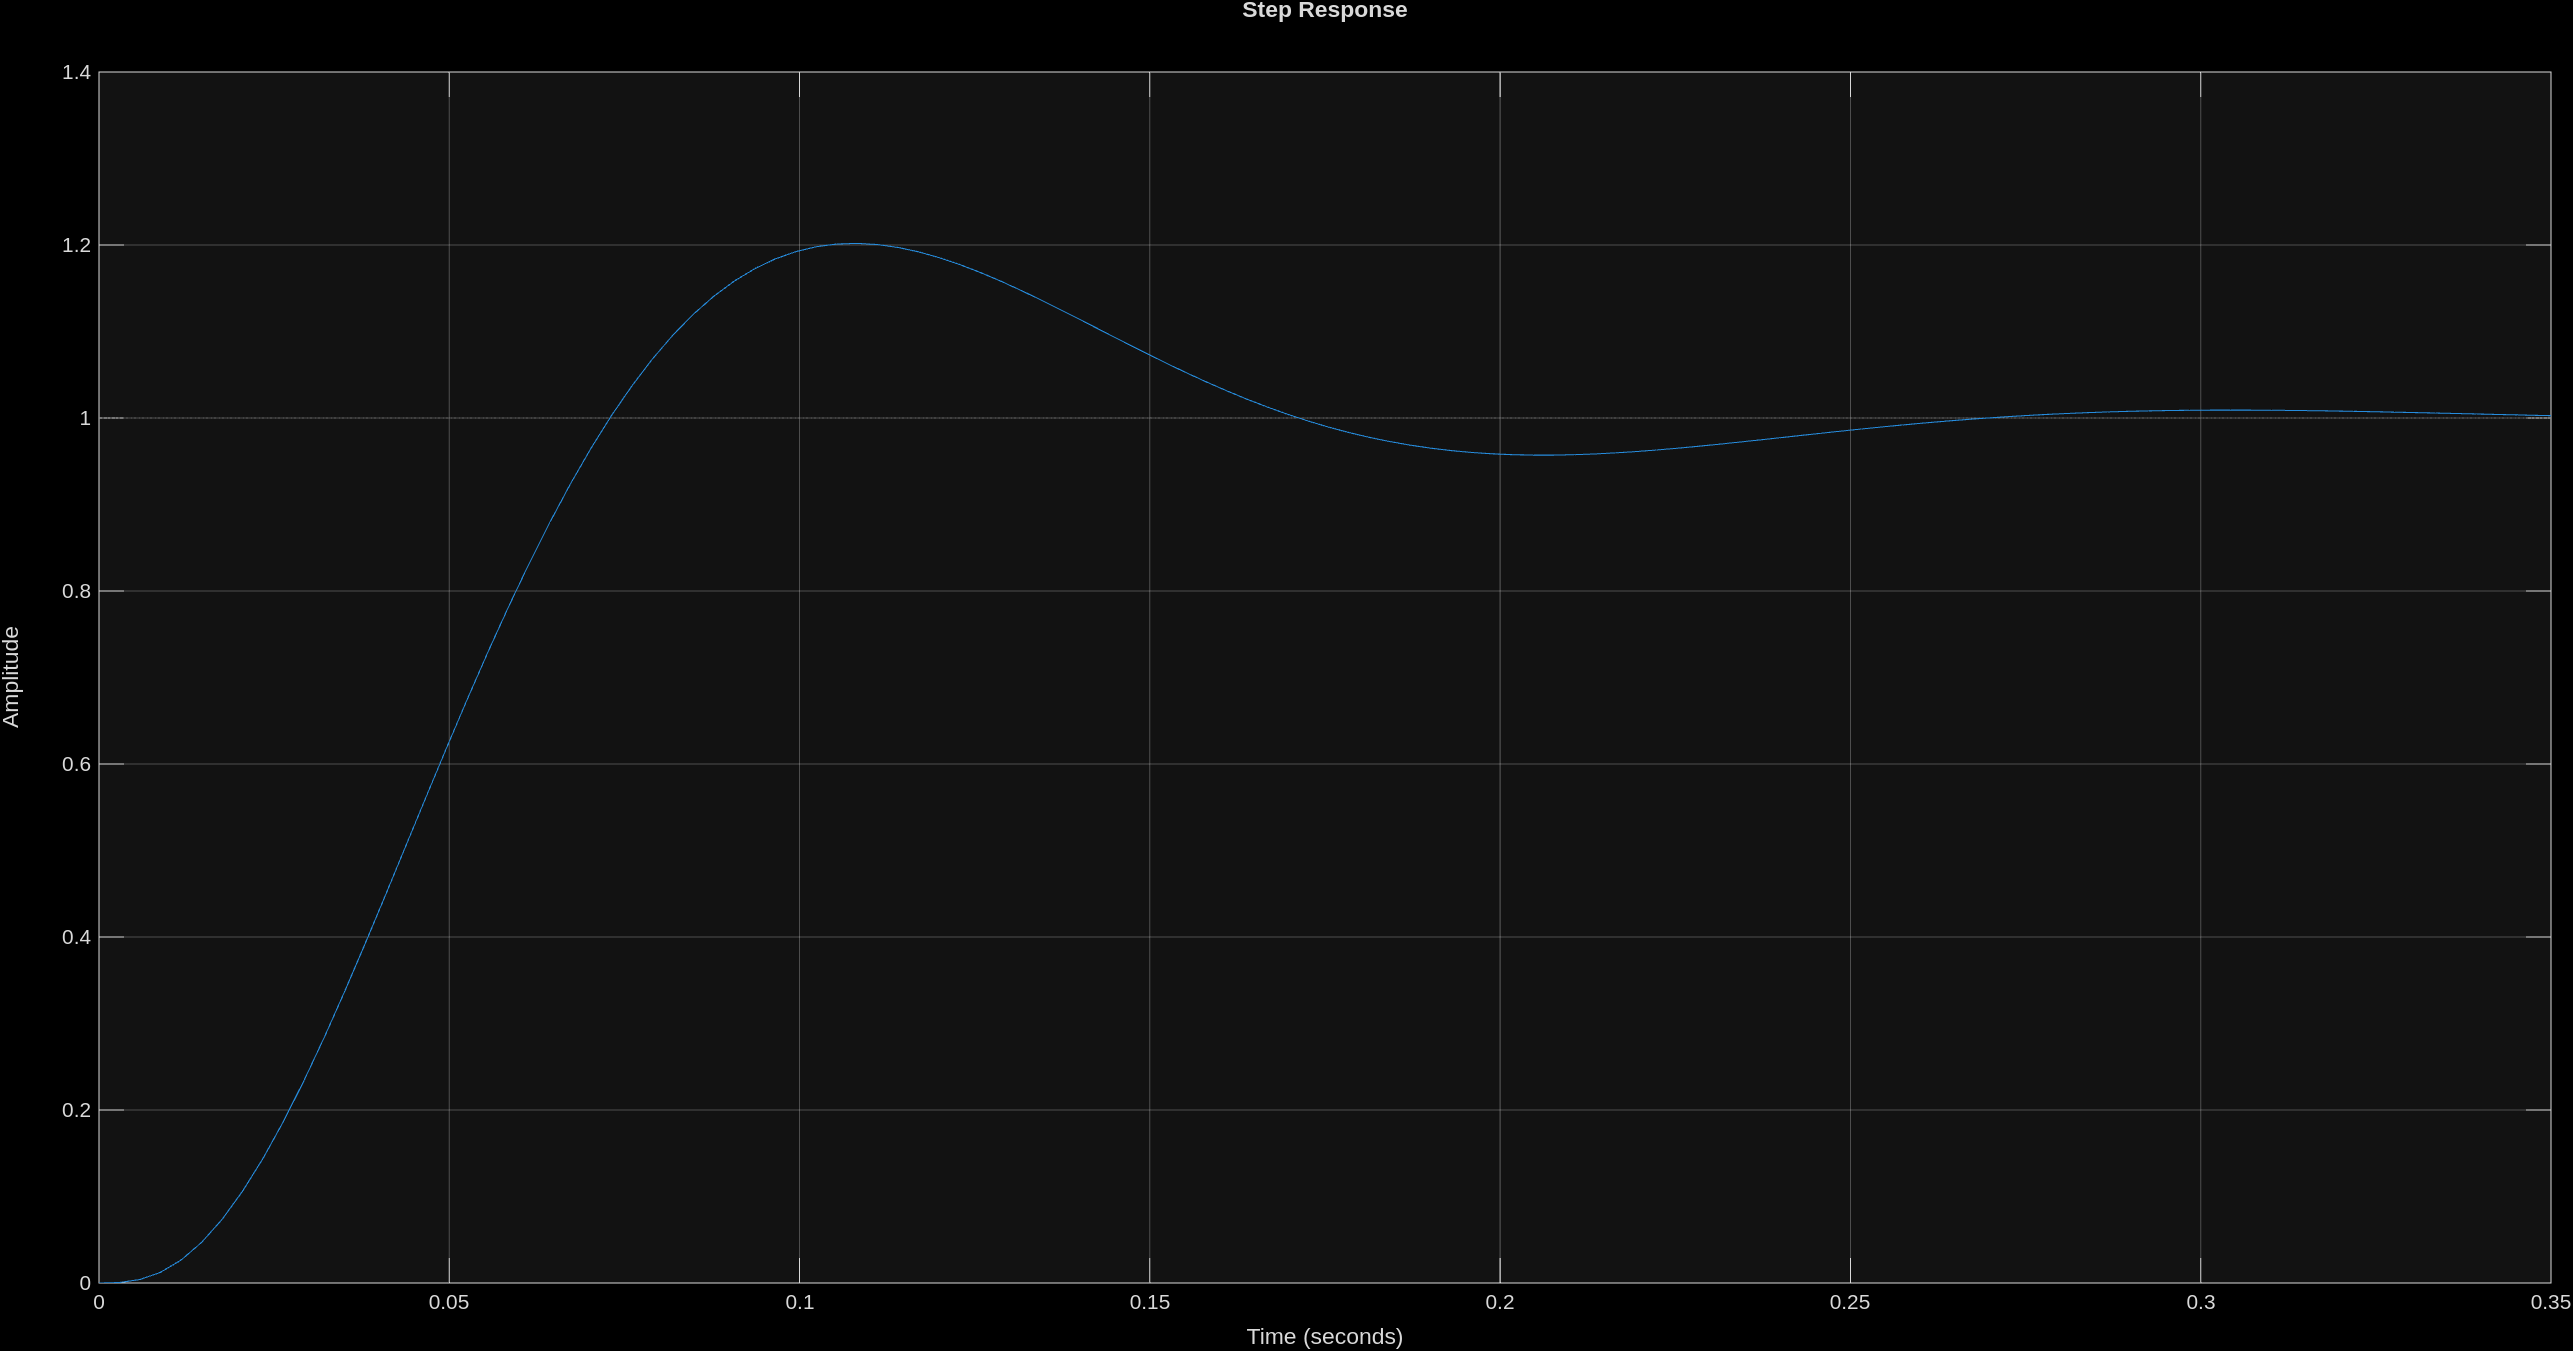
\includegraphics[width=1\textwidth]{step_response.png}
    \caption{step response}
\end{figure}

\section{Příklad 2}

\begin{figure}[H]
    
\includegraphics[width=1\textwidth]{notebook2.jpg}
    \caption{zápisky 2}
\end{figure}


\end{document}